\section{Historias de usuario}

Como metodología de desarrollo se escogió scrum. Esta nos permite tener avances
rápidos y modificaciones de las características de nuestro software en medio
del proceso de desarrollo. El seguimiento de estas características se lo hace
por medio de las historias de usuario, las cuales contienen el detalle
completo de la funcionalidad a ser implementada. Para crear las historias
de usuario se debe tomar en cuenta todos los detalles de la funcionalidad
y la estimación del esfuerzo necesario para completar la tarea (por medio
los puntos de la historia).

Como nombre del proyecto se escogió Loopify, la aplicación contempla
la creación de la aplicación web y un librería personalizada (Opal-Music) para
la generación de notas musicales. A continuación se detalla las historias
iniciales para la creación del proyecto.

\subsection{Aplicación Web (Loopify)}

La aplicación podrá generar loops por medio secuencias. Una secuencia representa
un sección con notas la cual puede repetirse múltiples veces a lo largo del loop.
Todas las secuencias tendrán una misma longitud de tiempo, lo que significa que
al agregar mas notas estas simplemente dividirán la secuencia por el numero de
notas requeridas, por lo que al agregar mas notas tendremos notas
de menor duración y al agregar menos notas tendremos notas con mayor duración.
Otra ventaja de tener secuencias con la misma longitud es que se vuelva mas
fácil secuenciarlas en el loop.

\subsubsection{Notas en una secuencia}

Para las notas de la secuencia se podrán escoger 1 2,4 u 8 notas.
(se escogieron pares para su división en partes iguales y para su uso interno
en la librería de edición musical). Al escoger el numero de notas se
crearan/disminuirán automáticamente el numero de dropdowns con notas.
En la tabla 3.1 se muestra un resumen de esta historia

\begin{table}[h]
\centering
\renewcommand{\arraystretch}{1.4}
\begin{tabular}{|*{4}{l|}}
\hline
\multicolumn{4}{|c|}{HISTORIA DE USUARIO} \\ \hline
NUMERO: & 108775342 & TIPO: & Feature \\ \hline
PUNTOS ESTIMADOS: & 2 & TÓPICO: & Editor Loops \\ \hline
TITULO: & \multicolumn{3}{|p{7.2cm}|}{Como cliente, puedo agregar notas a mi secuencia} \\ \hline
\multicolumn{4}{|l|}{DESCRIPCIÓN : } \\ \hline
\multicolumn{4}{|l|}{Se podrá cambiar las notas de una secuencia especifica} \\ \hline
\multicolumn{4}{|l|}{TAREAS : } \\ \hline
\multicolumn{4}{|p{11cm}|}{
\begin{minipage}[t]{\hsize}
  \begin{itemize}
    \item Agregar notas por medio del atributo 'notes' de 'sequence'
    \item Agregar select con opcion a 1,2,4 u 8 notas, guardar en la base en campo 'quantity' para agregar el tiempo en cada nota (1 = whole note, 2 = half note, 4 = quarter note, 8 = eighth note)
    \item Al escoger el numero de notas se debe desplegar el numero de selects respectivo (las cuales tendran como opciones las notas musicales existentes), por defecto empezara con una nota vacia o '-'
  \end{itemize}
\end{minipage}
} \\ \hline
\end{tabular}
\caption{Historia de Usuario: Como cliente, puedo agregar notas a mi secuencia}
\label{tab:Primero}
\end{table}

\subsubsection{Creación de múltiples secuencias}

Una ves creada la posibilidad de añadir secuencias debemos tener también la posibilidad
de crear otras para programarlas en el loop. Cada secuencia tendrá la posibilidad
de tener un tipo de efecto/timbre, un volumen determinado y la posibilidad de
escucharla por medio de un botón de reproducción
. En tabla 3.2 se incluye a mas detalle la implementación de
esta historia

\begin{table}[h]
\centering
\renewcommand{\arraystretch}{1.4}
\begin{tabular}{|*{4}{l|}}
\hline
\multicolumn{4}{|c|}{HISTORIA DE USUARIO} \\ \hline
NUMERO: & 106593214 & TIPO: & Feature \\ \hline
PUNTOS ESTIMADOS: & 2 & TÓPICO: & Editor Loops \\ \hline
TITULO: & \multicolumn{3}{|p{7.2cm}|}{Como cliente, puedo crear un loop con múltiples secuencias} \\ \hline
\multicolumn{4}{|l|}{DESCRIPCIÓN : } \\ \hline
\multicolumn{4}{|p{11cm}|}{Este editor permitira la creacion basica de loops, los cuales tendran mas de una secuencia} \\ \hline
\multicolumn{4}{|l|}{TAREAS : } \\ \hline
\multicolumn{4}{|p{11cm}|}{
\begin{minipage}[t]{\hsize}
  \begin{itemize}
    \item El usuario puede modificar el titulo y volumen del loop
    \item Crear boton de play que reproducir la secuencia
    \item Crear control de volumen
    \item Se puede añadir efectos para cada loop (usar tipo de onda de web audio API (sine, square, etc))
  \end{itemize}
\end{minipage}
} \\ \hline
\end{tabular}
\caption{Historia de Usuario: Como cliente, puedo crear un loop con múltiples secuencias}
\label{tab:Primero}
\end{table}

\subsubsection{Cambio de notas en el momento de la reproducción}

Con el fin de poder escuchar los cambios realizados a una secuencia, esta debe
tener la posibilidad de cambiar internamente sin interrumpir la reproducción,
la cual siempre se reproduce de manera continua, a menos que se haga stop
de la secuencia. Si se cambia una nota este cambio se vera reflejada en la siguiente
reproducción de la secuencia, sin tener que reiniciar su reproducción, como
se detalla en la tabla 3.3 esto debe realizarse junto con la
librería de edición creada

\begin{table}[h]
\centering
\renewcommand{\arraystretch}{1.4}
\begin{tabular}{|*{4}{l|}}
\hline
\multicolumn{4}{|c|}{HISTORIA DE USUARIO} \\ \hline
NUMERO: & 110280888 & TIPO: & Feature \\ \hline
PUNTOS ESTIMADOS: & 3 & TÓPICO: & Editor Loops \\ \hline
TITULO: & \multicolumn{3}{|p{7.2cm}|}{Habilidad para cambiar notas al momento de reproducirlas} \\ \hline
\multicolumn{4}{|l|}{DESCRIPCIÓN : } \\ \hline
\multicolumn{4}{|p{11cm}|}{Al momento de reproducir la secuencia, añadir la habilidad de cambiar las notas y que estos cambios estén presentes en la siguiente reproducción del loop} \\ \hline
\multicolumn{4}{|l|}{TAREAS : } \\ \hline
\multicolumn{4}{|p{11cm}|}{
\begin{minipage}[t]{\hsize}
  \begin{itemize}
    \item Añadir la habilidad de mutar las notas en el momento de reproducción
    \item Realizar estos cambios junto con la librería Opal-Music
  \end{itemize}
\end{minipage}
} \\ \hline
\end{tabular}
\caption{Historia de Usuario: Habilidad para cambiar notas al momento de reproducirlas}
\label{tab:Primero}
\end{table}

\subsubsection{Programación de múltiples secuencias en el loop}

Para programar las secuencias se creara una matriz gráfica de checkboxes, cada
fila representa a una secuencia y cada columna el instante en el que se las
reproducirá (si esta marcada se reproduce, sino simplemente se reproduce como
una secuencia en silencio). En la tabla 3.4 se detalle lo necesario para crear
esta historia

\begin{table}[h]
\centering
\renewcommand{\arraystretch}{1.4}
\begin{tabular}{|*{4}{l|}}
\hline
\multicolumn{4}{|c|}{HISTORIA DE USUARIO} \\ \hline
NUMERO: & 111056932 & TIPO: & Feature \\ \hline
PUNTOS ESTIMADOS: & 3 & TÓPICO: & Editor Loops \\ \hline
TITULO: & \multicolumn{3}{|p{7.2cm}|}{Habilidad para programar las secuencias por medio de una matriz gráfica} \\ \hline
\multicolumn{4}{|l|}{DESCRIPCIÓN : } \\ \hline
\multicolumn{4}{|p{11cm}|}{Se usara una matriz (gráficamente) para especificar el momento de reproduccion de una secuencia, cada fila representa una secuencia, las columnas son el punto de reproduccion de la secuencia, si se encuentra seleccionada esta sera reproducida, sino se lo toma como un espacio en blanco (no se reproduce)} \\ \hline
\multicolumn{4}{|l|}{TAREAS : } \\ \hline
\multicolumn{4}{|p{11cm}|}{
\begin{minipage}[t]{\hsize}
  \begin{itemize}
    \item Añadir una matriz de selects para programar cada una de las secuencias
    \item Añadir la posibilidad de aumentar o disminuir la longitud de todo el loop, lo cual aumentara o disminuirá el numero de selects en la matriz gráfica de reproducción
    \item Realizar estos cambios junto con la librería Opal-Music
  \end{itemize}
\end{minipage}
} \\ \hline
\end{tabular}
\caption{Historia de Usuario: Habilidad para programar las secuencias por medio de una matriz gráfica}
\label{tab:Primero}
\end{table}

\subsubsection{Usuarios con múltiples loops}

Una ves creada la posibilidad de tener un loop y programar nuestras notas por
medio de secuencias debemos poder tener la posibilidad de tener múltiples loops
por usuario. En la tabla 3.5 se detalla esta historia

\begin{table}[h]
\centering
\renewcommand{\arraystretch}{1.4}
\begin{tabular}{|*{4}{l|}}
\hline
\multicolumn{4}{|c|}{HISTORIA DE USUARIO} \\ \hline
NUMERO: & 109250002 & TIPO: & Feature \\ \hline
PUNTOS ESTIMADOS: & 2 & TÓPICO: & Usuario \\ \hline
TITULO: & \multicolumn{3}{|p{7.2cm}|}{Como usuario, puedo tener mas de un solo loop} \\ \hline
\multicolumn{4}{|l|}{DESCRIPCIÓN : } \\ \hline
\multicolumn{4}{|p{11cm}|}{El usuario podrá crear múltiples loops y visualizarlos en una lista} \\ \hline
\multicolumn{4}{|l|}{TAREAS : } \\ \hline
\multicolumn{4}{|p{11cm}|}{
\begin{minipage}[t]{\hsize}
  \begin{itemize}
    \item Crear pagina de indice para listar loops
    \item Añadir formulario para crear un nuevo loop
    \item Añadir habilidad de redireccionar al nuevo loop una ves creado
  \end{itemize}
\end{minipage}
} \\ \hline
\end{tabular}
\caption{Historia de Usuario: Como usuario, puedo tener mas de un solo loop}
\label{tab:Primero}
\end{table}

\subsubsection{Usuario puede copiar un loop}

Con el objetivo de tener un control de versionamiento cada usuario podrá
crear su propia versión de un loop especifico, para esto cada usuario
tendrá la posibilidad de navegar entre los listados de loops de otros
usuarios, pero solo podrán modificarlos si hacen una copia propia. En
la tabla 3.6 se resume esta historia

\begin{table}[h]
\centering
\renewcommand{\arraystretch}{1.4}
\begin{tabular}{|*{4}{l|}}
\hline
\multicolumn{4}{|c|}{HISTORIA DE USUARIO} \\ \hline
NUMERO: & 119350913 & TIPO: & Feature \\ \hline
PUNTOS ESTIMADOS: & 3 & TÓPICO: & Usuario \\ \hline
TITULO: & \multicolumn{3}{|p{7.2cm}|}{Como usuario puedo hacer una copia de un loop perteneciente a otro usuario} \\ \hline
\multicolumn{4}{|l|}{DESCRIPCIÓN : } \\ \hline
\multicolumn{4}{|p{11cm}|}{Un usuario podrá hacer copia de un loop perteneciente a otro usuario para realizar sus propios cambios} \\ \hline
\multicolumn{4}{|l|}{TAREAS : } \\ \hline
\multicolumn{4}{|p{11cm}|}{
\begin{minipage}[t]{\hsize}
  \begin{itemize}
    \item Añadir habilidad de navegar en la lista de loops de otros usuarios
    \item Agregar botón con texto 'Copiar a mi perfil'
    \item Al hacer click se añadirá una nueva copia de ese loop para el usuario que lo copio
  \end{itemize}
\end{minipage}
} \\ \hline
\end{tabular}
\caption{Historia de Usuario: Como usuario puedo hacer una copia de un loop perteneciente a otro usuario}
\label{tab:Primero}
\end{table}

\subsubsection{Agregar amigos}

Para tener una mayor visibilidad de nuestros loops se creara la posibilidad
de agregar a otros usuario como amigos, esto permitira ver las actividadades
realizadas por los usuarios en la tabla 3.7 se explica a mayor detalle la
historia

\begin{table}[h]
\centering
\renewcommand{\arraystretch}{1.4}
\begin{tabular}{|*{4}{l|}}
\hline
\multicolumn{4}{|c|}{HISTORIA DE USUARIO} \\ \hline
NUMERO: & 122381119 & TIPO: & Feature \\ \hline
PUNTOS ESTIMADOS: & 3 & TÓPICO: & Usuario \\ \hline
TITULO: & \multicolumn{3}{|p{7.2cm}|}{ Como usuario, puedo agregar otros usuarios como amigos} \\ \hline
\multicolumn{4}{|l|}{DESCRIPCIÓN : } \\ \hline
\multicolumn{4}{|p{11cm}|}{El usuario podrá agregar amigos y enterarse de sus actividades} \\ \hline
\multicolumn{4}{|l|}{TAREAS : } \\ \hline
\multicolumn{4}{|p{11cm}|}{
\begin{minipage}[t]{\hsize}
  \begin{itemize}
    \item Crear una lista de usuarios dentro de la aplicación
    \item Añadir botón 'Agregar como amigo' alado de cada usuario
    \item Crear pagina de noticias con las actualizaciones de los amigos agregados
  \end{itemize}
\end{minipage}
} \\ \hline
\end{tabular}
\caption{Historia de Usuario: Como usuario, puedo agregar otros usuarios como amigos}
\label{tab:Primero}
\end{table}

\subsubsection{Muro de actualizaciones}

Las actualizaciones son un punto importante para agregar la funcionalidad
de 'red social', para tener un punto de partida de visualización las actualizaciones
se creara un un muro de notificaciones donde se podrá ver a cada uno de nuestros
amigos y sus respectivas actividades, en la tabla 3.8 se detalla los
tipos de actualizaciones que tendrá la aplicación

\begin{table}[h]
\centering
\renewcommand{\arraystretch}{1.4}
\begin{tabular}{|*{4}{l|}}
\hline
\multicolumn{4}{|c|}{HISTORIA DE USUARIO} \\ \hline
NUMERO: & 122458919 & TIPO: & Feature \\ \hline
PUNTOS ESTIMADOS: & 3 & TÓPICO: & Usuario \\ \hline
TITULO: & \multicolumn{3}{|p{7.2cm}|}{Como usuario puedo revisar mi muro de notificaciones} \\ \hline
\multicolumn{4}{|l|}{DESCRIPCIÓN : } \\ \hline
\multicolumn{4}{p{11cm}}{El usuario recibirá actualizaciones especificas de sus amigos} \\ \hline
\multicolumn{4}{|l|}{TAREAS : } \\ \hline
\multicolumn{4}{|p{11cm}|}{
\begin{minipage}[t]{\hsize}
  \begin{itemize}
    \item Actualización cuando amigos agregan otros amigos
    \item Actualización cuando amigos crean nuevos loops
    \item Actualización cuando amigos copian otros loops
  \end{itemize}
\end{minipage}
} \\ \hline
\end{tabular}
\caption{Historia de Usuario: Como usuario puedo revisar mi muro de notificaciones}
\label{tab:Primero}
\end{table}

\subsection{Librería Edición Musical (Opal-Music)}

El motor de la aplicación web sera la librería Opal-Music, la cual permitirá la creación
y manipulación de notas y efectos musicales por medio de Web Audio Api.
Web Audio Api es un librería creado por Google para la manipulación de
sonidos en la web, funciona en cualquier navegador con HTML5.
Esta librería solo funciona con el lenguaje de programación JavaScript.
Con el objetivo de usarlo de manera mas fácil junto con la aplicación se lo creo
por medio de Opal, el cual es un transpilador que se encarga de transformar
código en el lenguaje Ruby al lenguaje JavaScript.

\subsubsection{Notas musicales con Web Audio Api}

Con el objetivo de abstraer la forma de crear notas se creara una clase llamada
'Note' la cual se encargara de crear notas con un volumen y una frecuencia especifica
(el numero de la frecuencia define la nota). En la tabla 3.9 se da mayor detalles
de esta historia

\begin{table}[h]
\centering
\renewcommand{\arraystretch}{1.4}
\begin{tabular}{|*{4}{l|}}
\hline
\multicolumn{4}{|c|}{HISTORIA DE USUARIO} \\ \hline
NUMERO: & 328 & TIPO: & Feature \\ \hline
PUNTOS ESTIMADOS: & 3 & TÓPICO: & Librería \\ \hline
TITULO: & \multicolumn{3}{|p{7.2cm}|}{Habilidad crear notas musicales por medio de la librería Web Audio API} \\ \hline
\multicolumn{4}{|l|}{DESCRIPCIÓN : } \\ \hline
\multicolumn{4}{|p{11cm}|}{Esta librería podrá generar notas musicales por medio de osciladores configurados a una frecuencia específica (relacionado con historia: 108775342)} \\ \hline
\multicolumn{4}{|l|}{TAREAS : } \\ \hline
\multicolumn{4}{|p{11cm}|}{
\begin{minipage}[t]{\hsize}
  \begin{itemize}
    \item Creación de sonidos por medio del oscilador de Web Audio API
    \item Especificar frecuencias para generar cada nota
    \item Modificación de la duración de una nota
    \item Modificación del volumen por medio de la amplitud de onda
    \item Modificación efectos por medio del tipo de onda
  \end{itemize}
\end{minipage}
} \\ \hline
\end{tabular}
\caption{Historia de Usuario: Habilidad crear notas por medio de Web Audio API}
\label{tab:Primero}
\end{table}

\subsubsection{Notas en secuencia}

La clase 'Sequence' podra crear multiples notas y secuenciarlas en un
determinado periodo de tiempo. El volumen y efecto de una secuencia
seran tambien configurados para cada nota. En la tabla 3.10 se
detalla la forma en que se manejaran notas vacias y la forma en la
que se secuenciaran las notas.

\begin{table}[h]
\centering
\renewcommand{\arraystretch}{1.4}
\begin{tabular}{|*{4}{l|}}
\hline
\multicolumn{4}{|c|}{HISTORIA DE USUARIO} \\ \hline
NUMERO: & 426 & TIPO: & Feature \\ \hline
PUNTOS ESTIMADOS: & 2 & TÓPICO: & Librería \\ \hline
TITULO: & \multicolumn{3}{|p{7.2cm}|}{Habilidad para reproducir notas en secuencia} \\ \hline
\multicolumn{4}{|l|}{DESCRIPCIÓN : } \\ \hline
\multicolumn{4}{|p{11cm}|}{Esta librería permitirá la reproducción de varias notas en secuencia (relacionado con historia: 108775342)} \\ \hline
\multicolumn{4}{|l|}{TAREAS : } \\ \hline
\multicolumn{4}{|p{11cm}|}{
\begin{minipage}[t]{\hsize}
  \begin{itemize}
    \item Programar una secuencia por medio de sus notas y duraciones
    \item Reproducir la siguiente nota al momento de terminarse la reproducción de la nota anterior
    \item Reproducir notas vacías como espacios silencios con una duración de tiempo
  \end{itemize}
\end{minipage}
} \\ \hline
\end{tabular}
\caption{Historia de Usuario: Habilidad para reproducir notas en secuencia}
\label{tab:Primero}
\end{table}

\subsubsection{Programación de secuencias}

Con el objetivo de repetir y/o programar una secuencia a lo largo del tiempo se
creara la clase 'Schedule' la cual se encargara de guardar y reproducir una
programación para una secuencia determinado. En la tabla 3.11 se detalla la
historia creada para esta característica

\begin{table}[h]
\centering
\renewcommand{\arraystretch}{1.4}
\begin{tabular}{|*{4}{l|}}
\hline
\multicolumn{4}{|c|}{HISTORIA DE USUARIO} \\ \hline
NUMERO: & 840 & TIPO: & Feature \\ \hline
PUNTOS ESTIMADOS: & 1 & TÓPICO: & Librería \\ \hline
TITULO: & \multicolumn{3}{|p{7.2cm}|}{ Habilidad para programar la reproducción de varias secuencias} \\ \hline
\multicolumn{4}{|l|}{DESCRIPCIÓN : } \\ \hline
\multicolumn{4}{|p{11cm}|}{Esta librería permitirá la programación de una secuencia a través de un tiempo determinado (relacionado con historia 111056932)} \\ \hline
\multicolumn{4}{|l|}{TAREAS : } \\ \hline
\multicolumn{4}{|p{11cm}|}{
\begin{minipage}[t]{\hsize}
  \begin{itemize}
    \item Crear un limite de duración
    \item En el limite provisto se repetirá la misma secuencia n veces o se omitirá su reproducción n veces en el limite de duración provisto
  \end{itemize}
\end{minipage}
} \\ \hline
\end{tabular}
\caption{Historia de Usuario: Habilidad para programar la reproducción de varias secuencias}
\label{tab:Primero}
\end{table}

\section{Interfaz De Usuario}

\subsection{Editor de loop}

El editor de loops a ser creado emulara el funcionamiento existente en
sequencers/trackers: una o varias pistas (secuencias) las cuales podrán
ser editadas y programadas en un punto del loop.
En la figura 3.1 podemos ver un primer ejemplo de como se visualizara un loop
junto con sus secuencias (representadas por medio de cuadros dentro de
la pagina). Cada secuencia tendrá los siguientes controles básicos: efecto,
volumen, botón de reproducción y cambio de titulo

\begin{figure}
  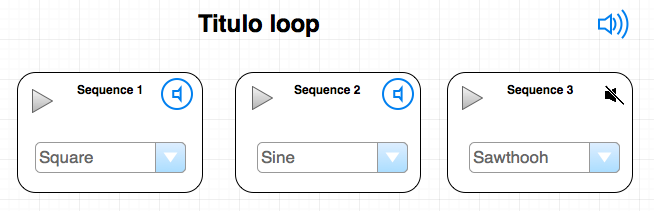
\includegraphics[width=\linewidth]{editor_con_secuencias.png}
  \caption{Editor con secuencias.}
  \label{fig:secuencia}
\end{figure}

Una ves creado los controles básicos del loop debemos crear los controles
que nos permitirán añadir notas a cada secuencia (ver figura 3.2). Para
esto se agregara un selector con el numero de notas deseadas. Por limites
del espacio de visualización para cada secuencia se limitara el numero de notas
a 8. Al escoger el numero de notas esta modificara dinámicamente los selectores
de notas dentro de cada secuencia

\begin{figure}
  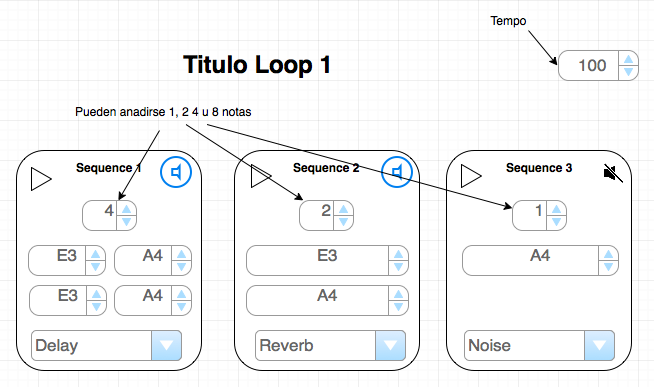
\includegraphics[width=\linewidth]{secuencias_con_notas.png}
  \caption{Secuencias con notas.}
  \label{fig:notas}
\end{figure}

Para la reutilización de las secuencias se creara una matriz de
programación (figura 3.3) encima de las secuencias. Cada fila representa una
secuencia y solo se reproducirá a lo largo del loop si la columna es
activada para su reproducción. A parte del boton de reproduccion para
cada secuencia se creara también un boton de reproducción para la matriz
programada

\begin{figure}
  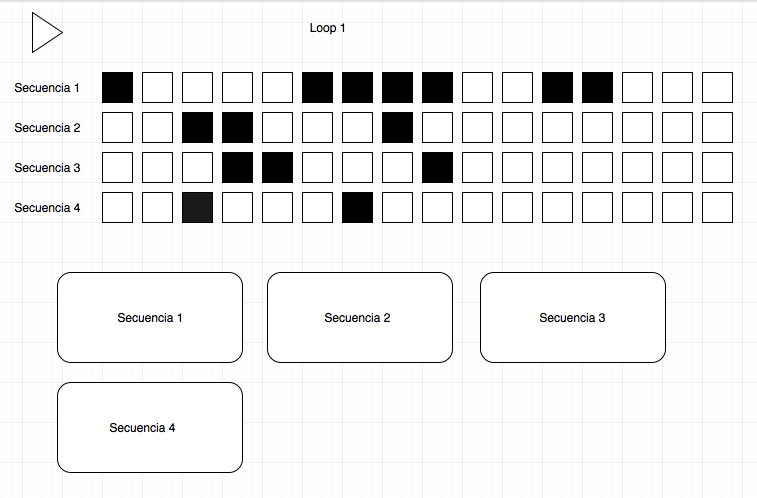
\includegraphics[width=\linewidth]{programacion_secuencias.png}
  \caption{Programación de secuencias.}
  \label{fig:programacion}
\end{figure}

\subsection{Usuarios}

Gran parte de la mecánica que nos permitira encontrar nuevos loops
se dara gracias a la interaccion entre usuarios. Como usuario podremos
crear, actualizar y eliminar nuestros loops como se muestra en la figura 3.4

\begin{figure}
  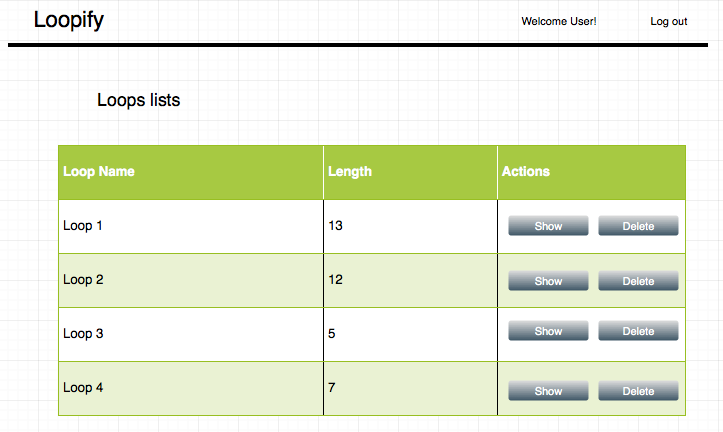
\includegraphics[width=\linewidth]{lista_loops.png}
  \caption{Lista de loops de usuario autenticado.}
  \label{fig:listaloops}
\end{figure}

También podremos descubrir y seguir las actividades de otros personas
dirigiéndonos al listado general de usuarios. Aquí podremos seguir un usuario
e incluso navegar entre los loops que han creado (figura 3.5)

\begin{figure}
  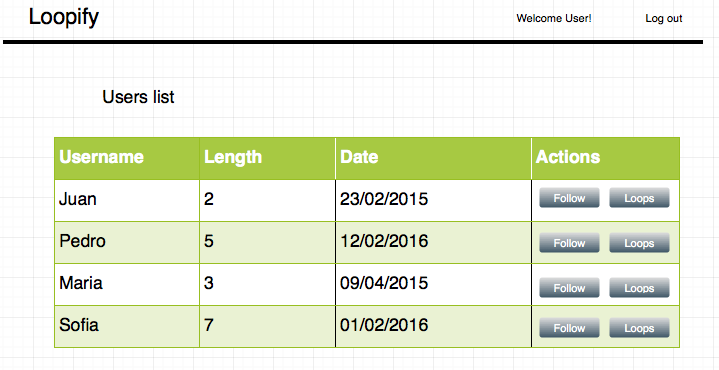
\includegraphics[width=\linewidth]{users_list.png}
  \caption{Lista de usuarios en el sistema.}
  \label{fig:listaloops}
\end{figure}

Dentro del listado de loops de otros usuarios (figura 3.6) solo podremos
hacer una copia del mismo, una ves copiados podremos modificarlos y
verlos dentro de nuestro lista de loops

\begin{figure}
  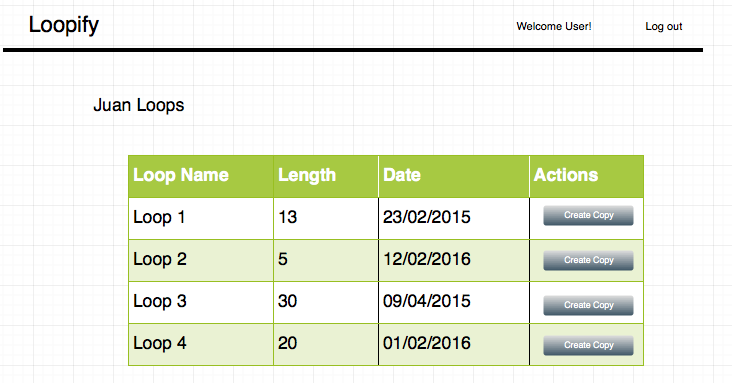
\includegraphics[width=\linewidth]{discover_loops.png}
  \caption{Lista de loops de otros usuarios.}
  \label{fig:listaloops}
\end{figure}

\subsection{Muro de Noticias}

Al agregar usuarios como amigos podremos ver sus actualizaciones dentro de
nuestro muro de noticias (figura 3.7)

\begin{figure}
  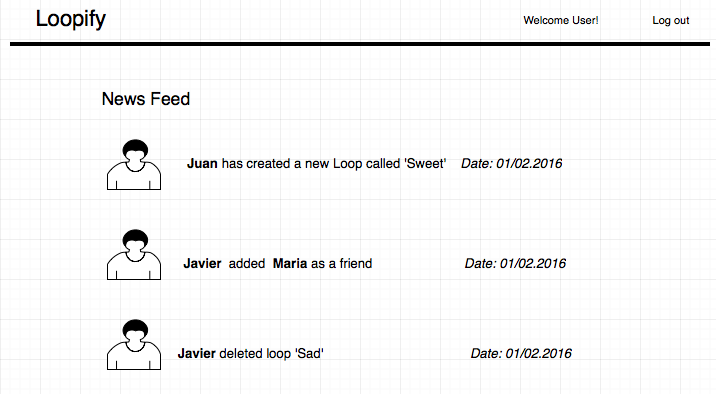
\includegraphics[width=\linewidth]{news_feed.png}
  \caption{Lista de noticias.}
  \label{fig:listaloops}
\end{figure}
